% 固定来源PDF印刷页52第19题两个正方形的示意重绘。
% 顶点关联及共边忠于原图，投影边长不代表空间角度的精确比例。
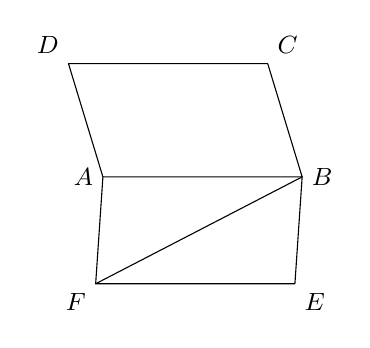
\begin{tikzpicture}[scale=1.15,line join=round,line cap=round,
  every node/.style={font=\small}]
\coordinate (A) at (0,0);
\coordinate (B) at (2.2,0);
\coordinate (D) at (-.38,1.25);
\coordinate (C) at (1.82,1.25);
\coordinate (F) at (-.08,-1.18);
\coordinate (E) at (2.12,-1.18);
\draw (A)--(D)--(C)--(B)--cycle;
\draw (A)--(F)--(E)--(B);
\draw (B)--(F);
\node[left] at (A) {$A$};
\node[right] at (B) {$B$};
\node[above left] at (D) {$D$};
\node[above right] at (C) {$C$};
\node[below left] at (F) {$F$};
\node[below right] at (E) {$E$};
\end{tikzpicture}
